\section{叠加与速度分析}
\label{sec:3.5}

按炮检距沿双曲线迸行叠加,可能是地震勘探中最重要的计算机处理过程了。比它偏移
更为重要,因为它使数据库从$(s, g, t)$空间的一个体积简化为$(y, t)$空间的一个平面。
地震资料解释人员现在还很少有人采用计算机化的电影式地震资料,所以大多数解释人员在
他们能解释分析之前都必须使地震资料经过叠加处理。偏移只不过就是把资料从一个平面转
换至另一个平面。此外,偏移有个缺点:有时它把近地表速度横向变化和多次反射造成的混
乱也混杂在一起了。叠加处理也可能混杂有这类影响,不过,在条件恶劣的地区,资料要不
经过叠加处理,那就别想看出什么东西。除前面列举的各点之外,叠加处理还有个附带的产
品,那就是据此可以估计岩石速度。

从历史上说,曾经采甩射线法来完成叠加处理,而且现在仍然几乎是唯一地按这种方式来
处理。而另一方面,偏移则总是采用波动方程方法来完成,那就是说,以Fourier变换或有
限差分方法来实现。偏移与叠加二者均属涊曲线识别处理过程,偏移时采用波动方程方法有
许多好处,这些好处难道不能同等地适用于益加吗?看起来似乎是应该如此,但是现在的勘
探实践还没有怔实这点,其原因还不太清楚。本章以后各节内容实际上是属于专题研究性
质,其标题不紡戏称为《不久将要建立的理论》。有关速度估计的更高级概念在\ref{sec:5.0}节至\ref{sec:5.4}
节讨论。波动方程叠加与速度测定方法均是独创性方法,它们也许还缉有经受过令人满意的
检验,或者它们也许还只是不完善地被汇总在一起的。给读者留有想像的余地,时间将会告
诉我们究竟如何。

为什么许多这种理论并没在常规勘探工作中应用?可能的一种原因是:为消除冗余信息
而进行叠加这种论点大概更适合于作为一个统计问题来处理,而不能作为一种物理问题来处
理。为考虑到这类随机偶然性,我得多用一点笔墨来讨论“波动方程时差校正”,这是一种
将统计分析推迟到向下延拓处理之后再迸行的方法。另一种可能原因则是:比起波动方程
来,用射线法解决:排列末端数据丢失和雄列长度范围内出现空间假频的问题,大概要更为灵
活。对于这类随机偶然性质,我特意列了简短一小节来讨论数据恢复问题。不论是哪种情
况,本章论述的数据处理办法想来都应有所裨益。

\subsection{正常时差校正(NMO)}
\label{sec:3.5.1}

正常时差校正(NMO)就是对时间轴进行某种拉伸,使所有地震记录看来像是零炮检
距地震记录。\ref{sec:3.0.1}节内曾首先讨论过NMO,在那种最简单的形式中,NMO是以毕达哥拉斯
关系$t_{nmo}^2=t^2-x^2/v^2$为基础的。在地层的速度为恒定时,正常时差校正要取双曲线族的渐
近线并沿它移动直至与$t=0$重合,这就是在时间轴上舍去初至之前的任何采样值,然后再将
地震记录的其余部分拉平。接近初至之处,拉伸影响最为显著,在以后的各时间上则逐次减
弱。在图\ref{fig:vdmo/cmpnmo}所示的正常时差校正例子中,你会注意到有由拉伸而形成的许多低频成分。
\begin{figure}[H]
\centering
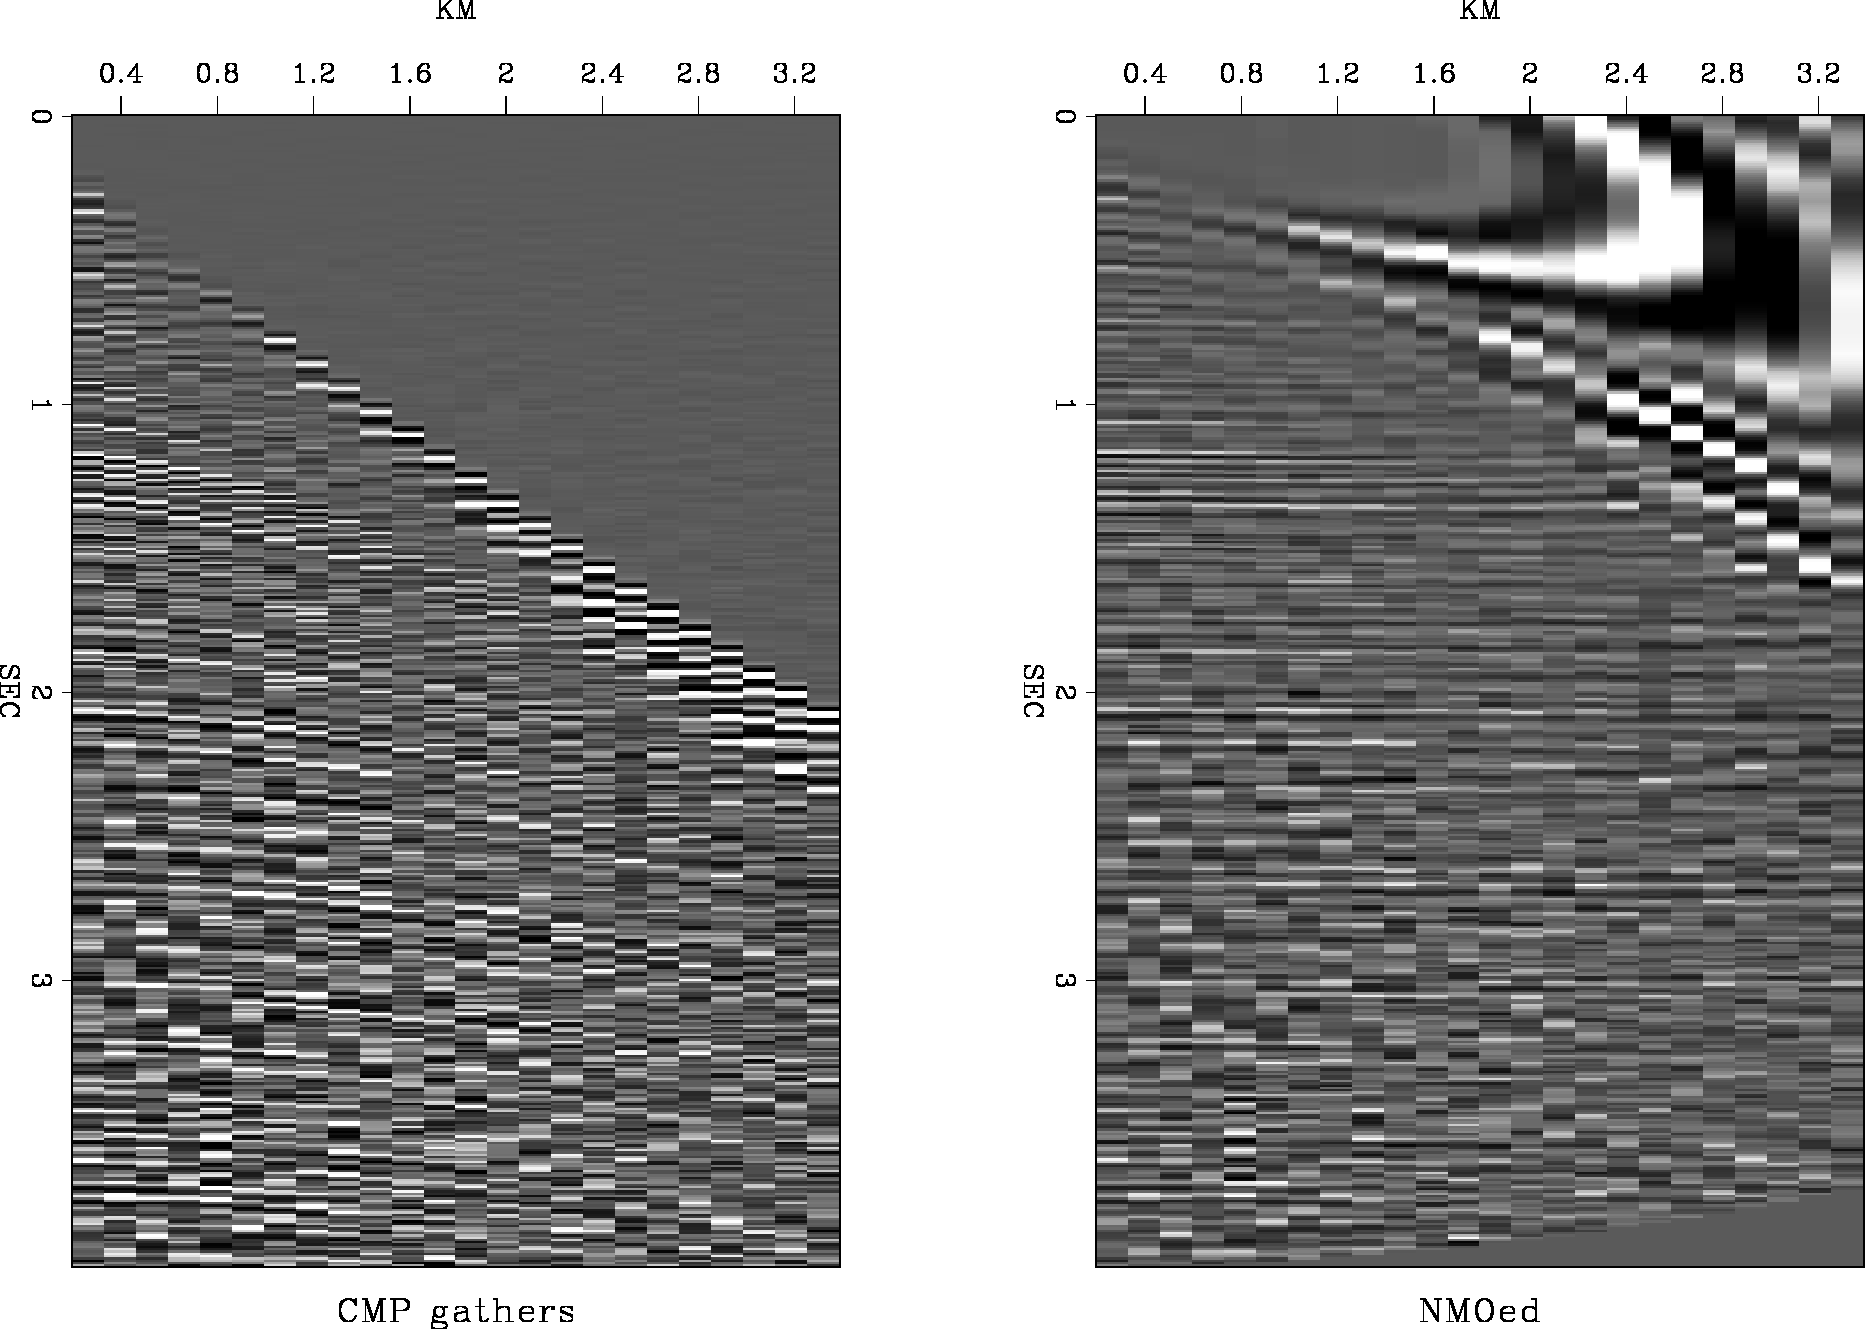
\includegraphics[width=0.65\textwidth]{vdmo/cmpnmo}
\caption[cmpnmo]{左图所示为墨西哥海湾地区的共中心点道集,经正常时差校正后如右图所示}
\label{fig:vdmo/cmpnmo}
\end{figure}

能够作正常时差校正的是共炮点道集或共中心点道集。应用于共炮点道集的正常时差校
正使该道集成为类似于零炮检距时间剖面的一小部分,这时地质构造突出地被展现出来。对共
中心点道集进行正常时差校正,是确定地层的速度与深度之函数关系的主要手段,这是因为共
中心点道集对地层之倾角是不灵敏的。

从数学上说,有关正常时差NMO的变换是一种线性运算。事情看来似乎有些矛盾,一种
非均匀的时间坐标拉伸运算竟是某种线性运算,可是坐标拉伸确实是满足与线性性质有关的
数学条件。不要把流行的线性条件混淆为不太常见的时间不变量条件。线性性质仅要求;对
于将原始数据P分成几部分(例如分成与$P_1$与$P_2$)的任何分解来说,经过正常时差校正的几
部分之和应等于和之正常时差校正。分解的例子包括:(1)分成较早各时间和较晚各时间;
(2)分成偶数时间点和奇数时间点;(3)分成高频和低频;(4)分成大信号值与小信号值。

为把正常时差校正想像成是一种线性算子,试将地震记录考虑为某种向量。NMO算子
类似于一个对角线矩阵,但是沿矩阵对角线分布的是内插滤波因子,而且各内插滤波因子均
有偏离对角线的相移以形成所期望的时延。

\subsection{常规速度分析}
\label{sec:3.5.2}

常规速度分析要利用一系列试验速度,每种试验速度取为深度的恒定函数并用它对数据
进朽时差校正。图\ref{fig:vdmo/cmphale}的左图为用一恒定速度对图\ref{fig:vdmo/cmpnmo}
所示共中心点道集进行时差校正之后的结果。注意,该道集中部的各同相额均将近拉平,而较小时间上的同相轴则校正不足,
较大时间上的同相轴则过校正。这种现象很典型,因为正常时差校正量的变化是与速度
呈反比关系(根据毕达哥拉斯关系即可知),而地层的速度在通常情形下正是随深度而增大
的。利用遍及CDP道集各炮检距进行求和的结果作为时差校正速度是否良好拟合于地层速度
的一神测度,大概说来,速度拟合程度越佳,求和值就将越大,用许多种速度重复进行这种
过程,按求和值的幅度绘制等值线图,将它显示为时间与速度的函数,这就是速度谱,如图
\ref{fig:vdmo/cmphale}的右图所示。

\begin{figure}[H]
\centering
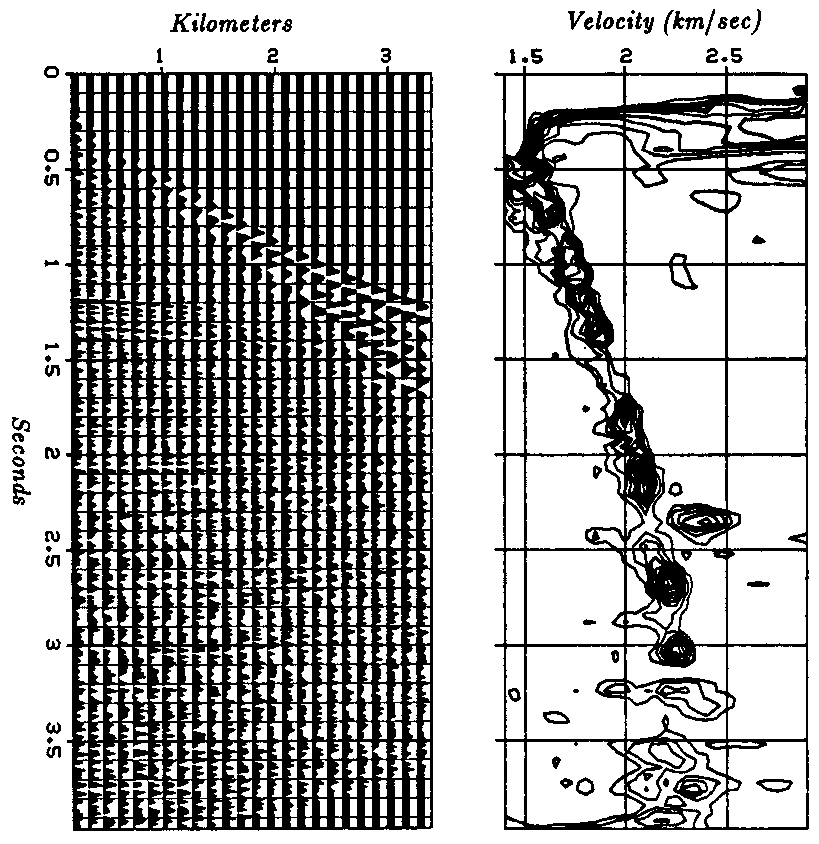
\includegraphics[width=0.65\textwidth]{vdmo/cmphale}
\caption[cmphale]{按恒定速度进行正常时差校正及速度分析结果}
\label{fig:vdmo/cmphale}
\end{figure}

在实际处理时,求和之前可
以采用一些额外的修饰处理步骤。可以按记录道的功率和按它
们的谱(见\ref{sec:5.5}节有关反褶积处理的论述)对各记录道作道间均
衡处理(使它们比例相等)。类似还有,可以将求和所得幅值加
以平滑和归一化(见Taner与 Koehler(l969)的论文)。还可
以如下节所述将数据加以编排和加权。

得出最佳叠加效果的速度是 反射面以上各地层之速度的某一
种平均值,这种平均值的精确定义推迟到\ref{sec:5.4}节再去讨论。

\subsection{切除与加权}
\label{sec:3.5.3}

定义切除函数是常规赴理中
的重要一部分。切除函数就是用 于压制掉数据中某些不希望要的
部分时所使用的一种加权函数。图\ref{fig:vdmo/mute}所示是经过切除处理之野外剖面的例子。加权与切
除对叠加的质量有重大影晌。因此,有许多试验和理论讨论实际上都是以它们作为研究主
题,这是毫不奇怪的。

\begin{figure}[H]
\centering
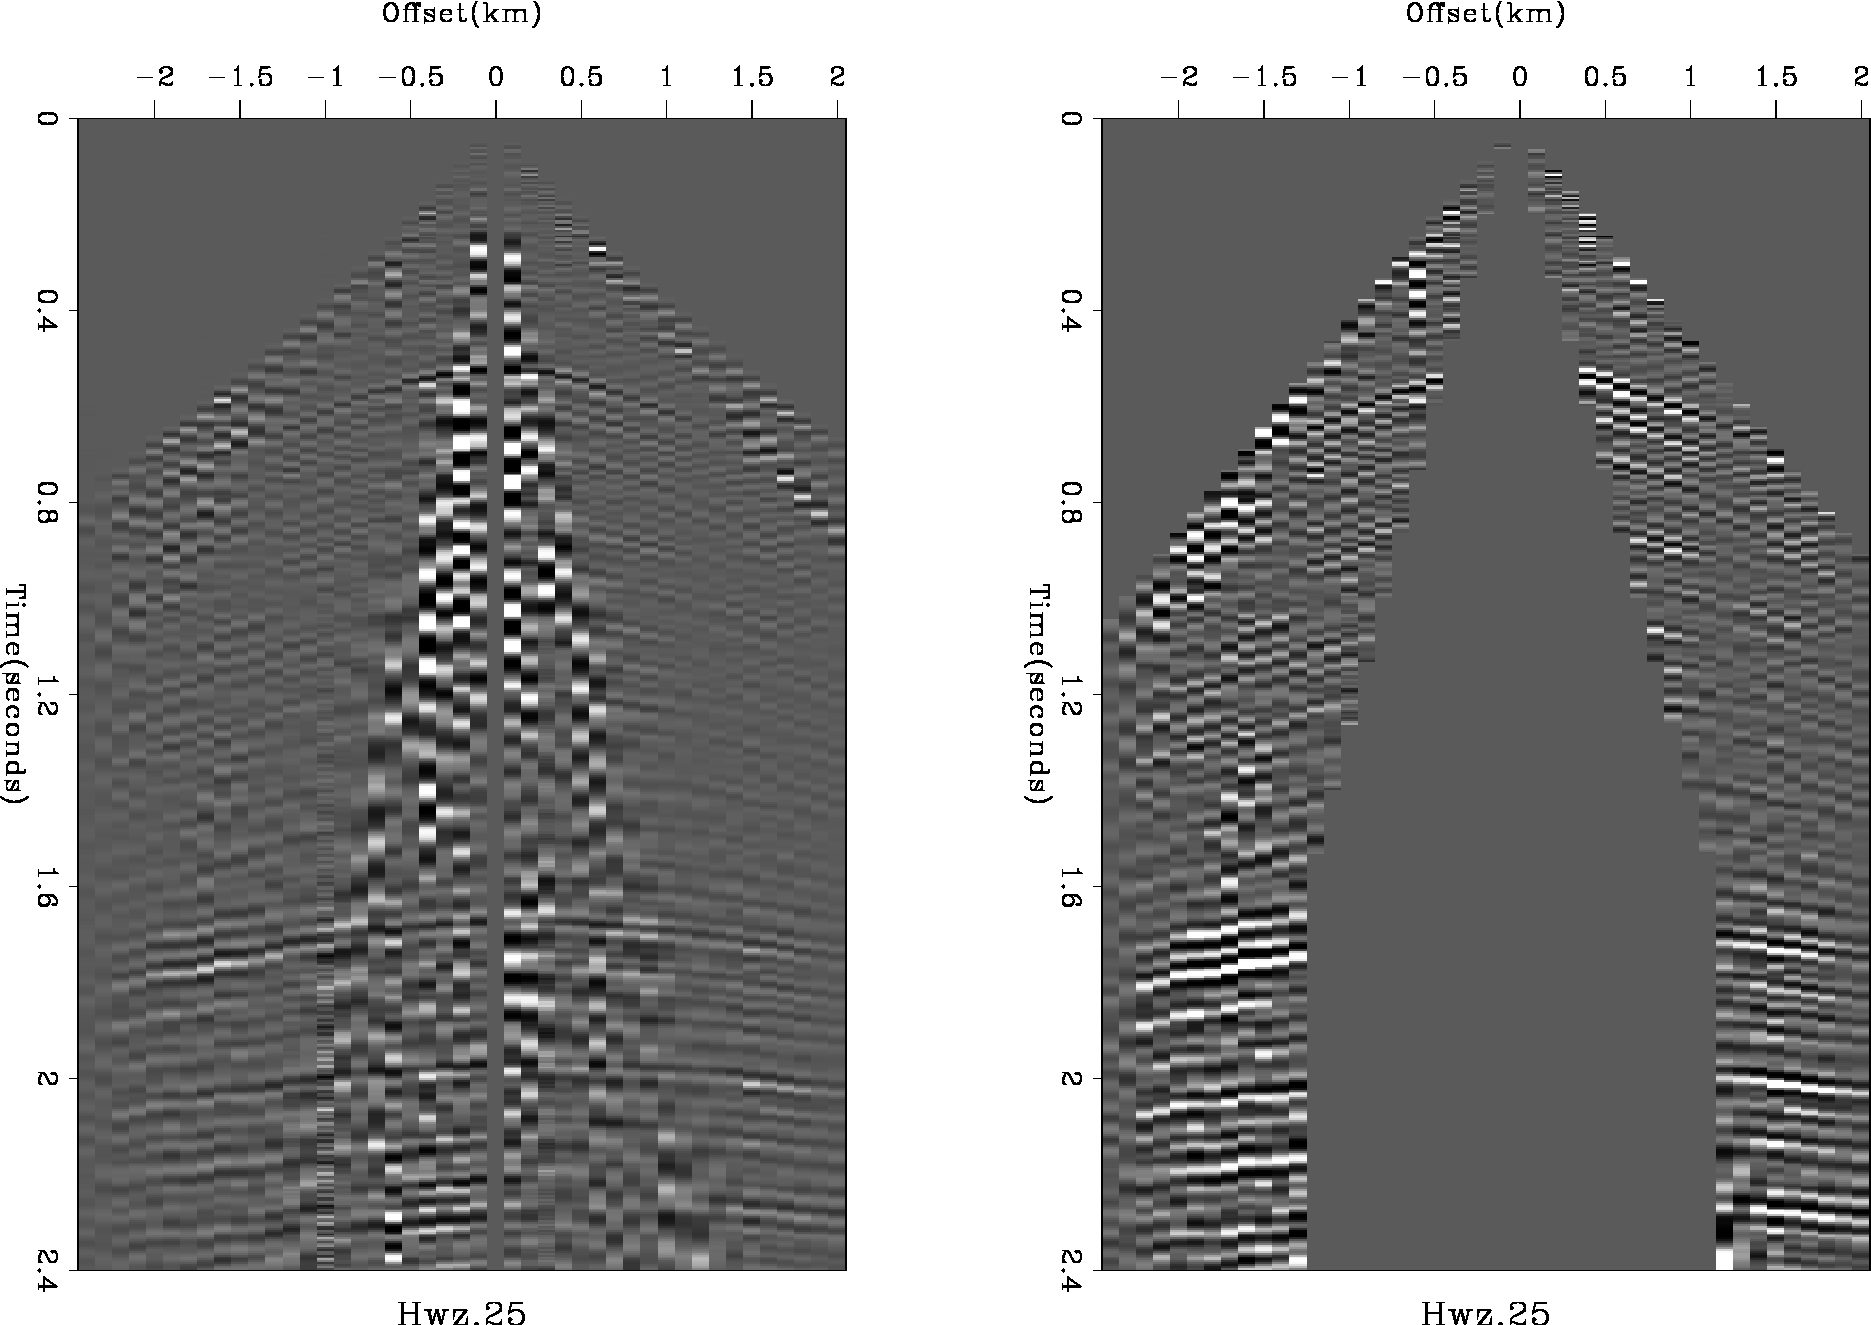
\includegraphics[width=0.65\textwidth]{vdmo/mute}
\caption[mute]{左图是Alberta地区的陆地勉震记录,右图是该记录经过切除处理后
的结果,地滚波(记录中部)与首波(第一个波至)均已消除}
\label{fig:vdmo/mute}
\end{figure}

切除函数往往是以r为变量的一维函数,其中\footnote{h为炮检距,t为时间.------译者},$r=h/t$。
既切除大r值时的数据也切除小r值时的数据,其原因如下所述。

在小r值时,炮点附近仍然可发现有能量存在,诸如水或泥块坠落所形成的影响,或者
低速地滚波所形成的干扰能量。

r值大时,则存在与初至有关的问题。在这种情形下,正常时差拉伸最大而且对速度极
敏感。这初至往往称作首波或折射波。从野外观测看,首波就是一种其旅行时间表现为距离
之线性函数的波。就理论上考虑,针对分层介质很容易对首波作出解释。首波具有沿一地层
边界面作水平传播的射线。在实际现象中,首波可以弱于或者是强于反射波,首波强于反射
波可以用反射波作三维分布而首波仅作二维分布这个事实来解释。

可以把切除楚理看作是用零值迸行加权。为产生最有利的叠加效果,可以选择更普遍性
的加权办法。完善的分析肯定应将干扰噪音和截断影响考虑在内,我们权且作一个简化分析
吧,它可导出最基本的加权函数。

一般我们是沿双曲线遍及所有炮检距进行求积。考虑三维问题时则与此不同,你这时实
际是希望遍及一旋转双曲面进行求积,假设该双曲面是呈径向对称的,按炮检距h的大小对
被积函数进行加权,就使得通常的线性积分能够模拟出遍及旋转双曲面的积分结果
\footnote{这是必须迸行加权处理的第一个理由.所谓沿双曲线的积分,实即正常时差校正并叠加;所罚沿旋转双曲面求
积,就是考虑球面扩散影响时的叠加。因此,必须按炮检距的大小,成比例地对叠加道(所谓被积函数)进行加权,校正
该种影响,这时的叠加处理(所谓的线性积分)结果,才能消除三维情形下的能量扩散。直接了当地说,进行加权处理的
第一个理由就是必须对波阵面球面扩散影响进行适当的补偿。}。叠加
前要按炮检距h的大小对数据进行按比例放大,还有第二个原因,那就是在零炮检距附近能
获得的速度信息不多,这些记录道的时差很小而在远炮检距时则可获得很多速度信息,这些
记录道的比值比较大
\footnote{这是必须进行加权处理的第二个理由。浅显地说,近炮点记录道时差小,因而速度分辨率低;远炮点记录道时差
大,速度分辨率高。但是近炮点记录道振幅强,而远炮点记录道因能量衰减而振幅弱,采用以叠加方法为基础的速度分析
时,将因此而主要是反映近炮点记录道的作周和影响,降低了速度分析的精度。因此必须按炮检距的大小而成比例地加权
放大记录道辐值,使得近炮点与远炮点记录道的振幅在叠加中发挥同等作用。这种加权处理,对远度谱而言,可提高速度
分辨率;对叠加处理来说,可提高叠加效果和质量。----译者}。

\subsection{NMO(正常时至校正)方程}
\label{sec:3.5.4}

在任一已知记录资料的深度范围之内,地层速度变化范围可达2倍左右,是很典型的情
形。这样一来,对于以毕达哥拉斯关系为基础的分析方法就得需要重新加以考虑砑究了。在
实际处理中,总是采取在毕达哥拉斯关系中插入一个随时间而变的速度这种办法来处理随深
度而变的速度(有关的经典参考文献见Taner与Koehler[l969]的论文,它包括有许多颇有
助益的细节讨论)。尽管计算正确的非双曲线时差校正并不困难,很多还是采用这种近似。
让我们看一看倒底是如何在数学上将速度函数$v(z)$同正常时差联系起来的。设共中心点道
集之一记为$P(h,t)$,正常时差校正将该CMP道集转换为某一地层模型$Q(h,z)$
\begin{equation}
Q(h,z)=earth(z)\times const(h)
\label{eq:ex3.5.1}
\end{equation}
实际上,$Q(h,z)$终究还不是$h$的恒定函数,它还只是我们所欲达到的目标。

可以把正常时差校正处理看成是一种简单的复制过程。这点在概念上很容易想像,它就
是把$(h,t)$平面上的每一个点复制拷贝到$(h,z)$平面上的适当位置。可将这一类拷贝过程记为
\begin{equation}
Q[h,z(h,t)]=P(h,t)
\label{eq:ex3.5.2}
\end{equation}
这么拷贝时,必须小心避免在$(h,z)$平面上留下一些空洞
\footnote{正常时差校正值需为时间采样间隔$\Delta t$的整涪数,但应校正的值不一定诒为其整数倍。在校正处理过程中,
超过整数倍之余值累积到等于一个$\Delta t$值时,须进行内插。所谓“空洞”,即应内插之处。----译者}。
最好是对$(h,z)$输出平面
内的每一个点迸行扫描,从而从$(h,t)$平面内找出其在$(h,z)$平面内产生该空洞的根
源。利用某种动校正时间表$t(h,z)$,可采取下列拷贝处理过程,对数据加以时差校正
\begin{equation}
Q[h,z(h,t)]=P[h,t(h,z)]
\label{eq:ex3.5.3}
\end{equation}

如采用本书的术语,时差校正处理的输入数据$P(h,t)$被称作CMP道集(共中心点道
集),而输出数据Q则被称作CDP道集(共深度点道集)。

在实际处理中,生成该旅行时间表的第一个步骤是把深度变量变成一垂直旅行时间变
量$\tau$。所以,所要求的表是$t(h, \tau)$,为得到位于$(h, \tau)$
的输出数据,你得在位置$(h,t)$
上取输入数据。产生这种时间表的最直接而可靠的途径,看来得按$z$的步长向下推迸。实际
也就是按$\tau$的步长向下推进,并沿射线追踪。那就是说,你要针对Snell参量$p$的各种固定值,
采用对下列两项方程遍及$\tau$迸行积分的办法根据$v(\tau)$计算出必$t(p,\tau)$和$h(p,\tau)$来
\begin{equation}
\frac{dt}{d\tau}=\frac{dz}{d\tau}\frac{dt}{dz}=v\frac{1}{vcos\theta}=\frac{1}{\sqrt{1-p^2v(\tau)^2}}
\label{eq:ex3.5.4}
\end{equation}
\begin{equation}
\frac{dh}{d\tau}=\frac{dz}{d\tau}\frac{dh}{dz}=vtan\theta=\frac{pv(\tau)^2}{\sqrt{1-p^2v(\tau)^2}}
\label{eq:ex3.5.5}
\end{equation}
在式\ref{eq:ex3.5.4}与式\ref{eq:ex3.5.5}中,$dt/dz$和$dh/dz$的表达式均是以射线为基础而不是以波阵
面为基础。给定了$t(p,\tau)$和$h(p,\tau)$,为消去$p$然后求出$t(h,\tau)$,需要进行叠代及内插方
法。这听上去挺难处理的---事实确实也是如此---因为在大角度时通常存在有到达反射
同相轴中部的首波,不过,一旦完成了这项工作,你就能存该表而多次重复利用它了。各
时距曲线在大炮检距上出现交叉分支现象,推动了以波动方程为基础的速度分析方法的建
立,最大的速度灵敏度正是出现在传统的双曲线假设初单一初至假设均不成立的那些地方。


\subsection{线性性质与统计估计}
\label{sec:3.5.5}

波动方程数竭处理方法具有的线性性质使柺我们能将数据集分解成儿部分,对每部分分
别地处理,然后将它们重新组合,所得结果同未作分解时处理所得结果相同。

例如,设把共中心点道集分成两部分,比如,分成近记录道部分A和远记录道部分B。
令$(A,0)$表示各远记录道均已置零的共中心点道集,$(0,B)$可以是该道集的另一拷
贝,其中各近记录道均已置零。我们可将$(A,0)$向下延拓,然后再独立地将$(0,
B)$向下延拓。在各自完成向下延拓之后,可将$(A,0)$与$(0,B)$相加起来。我们可以轮流地
暂停延拓,就统计姓理作出某神考虑,然后选择用某种加权函数把它们组合起来。图\ref{fig:vdmo/decomp}
所示为三个记录道组成的数据集被分解成三个数据集,每道就是一个数据集,图中的半圆是
各记录道单独进行向下延拓时的扫描路径,每个半圆都通过零炮检距,给岀已适当展乎、经
过正常时差校正之后的记录道\footnote{这就是本书所谓的“波动方程时差校正”,实际就是叠前偏移。 ---译者}。

\begin{figure}[H]
\centering
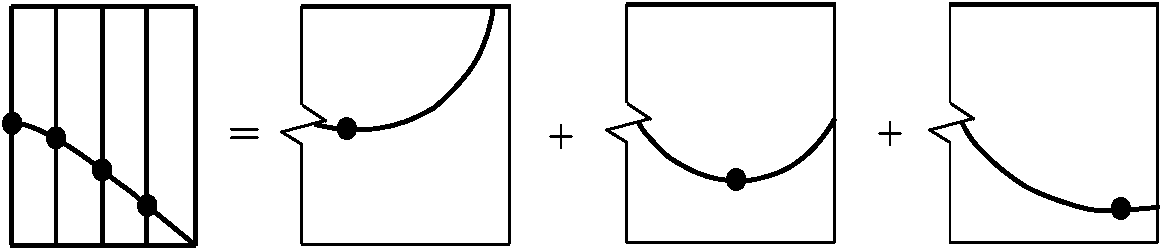
\includegraphics[width=0.65\textwidth]{vdmo/decomp}
\caption[decomp]{三个记录道组成的共中心点道集按各记录道分解成三部分
左端,资料中的豚冲经过内插处理,可描绘出一双曲线轨迹。右端,各数据点均扩展成偏移半圆,
各半圆均通过位于双曲线顶点的零炮检距}
\label{fig:vdmo/decomp}
\end{figure}

采用加权函数这神思想,极端不同于我们先前进行分析的风格,它代表一种干扰识别的
概念,这是我们始终忽略了的在所有科学分析中都很重要的某种东西,那就是统计方法!是
什么因素要求选择一种加权函数呢?因素有很多,信噪比是起作用的一种因素;某些记录道
可能受噪音干扰或缺失,也是因素.当斟酌最终显示形式时,必须考虑人的感觉能力,并且
需要压缩动态范围,以便很小的值也能被发现.不但在明显易见的$(h,t)$空间内,而且在
频率域、倾角域或者在可能使波场过于超出均衡状态的任何其他空间内,都必须考虑动态范
围的压缩问题。

分解数据集有许多种方法,究竟选择何者,这决定于你的统计模型和你是否愿意使处理
重复进行许多次。也许数据道集的几部分不应该按其炮检距$h$来分解,而只应按它们的$r=h/t$
的值来分解。显然,要考虑的问题是很多的。

% \subsection{正向与反向散射:Larner条痕}
% \label{sec:3.2.6}

% 在某些地段上,远地表波(near-surface wave)压制了有地质意义的深层反射。由于
% 地表面比起下面较深地层更为大大地不规则,所以近地表波通常均不规则,这使得我们的困
% 难复杂化了。在陆地上,这些干涉波称作地滚波;在海上,它们称作水波(water wave),
% 但别把它们与水面上的表面波相混。

% 图\ref{fig:ofs/vertlay}中垂直的反射壁就可能是产生这类近地表干扰的一种模型,在这种模型中,波
% 仍然是靠近地表传播的。随机分布的垂直壁可以形成类似图\ref{fig:ofs/shelikof}所示野外资料那样的零炮
% 检距时间剖面。另一类不太少见的近地表干扰模型就是随机点散射模型中的平顶曲线了。

% \begin{figure}[H]
% \centering
% 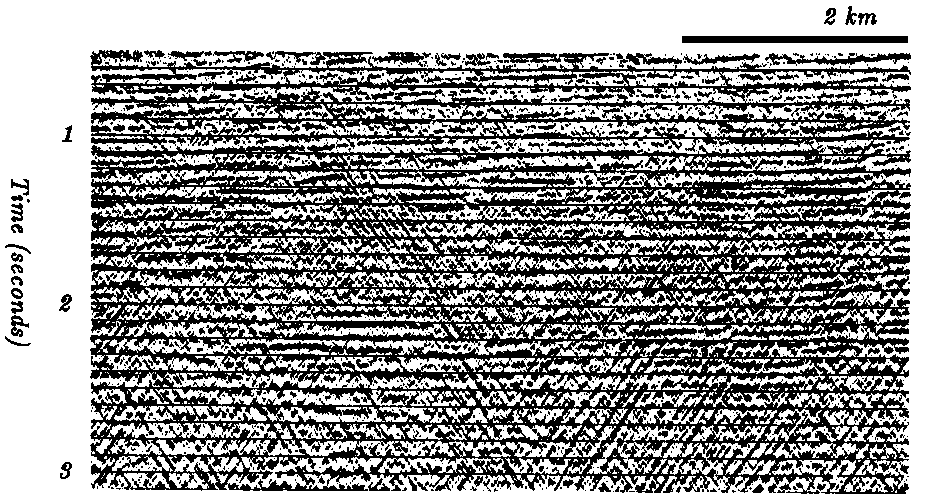
\includegraphics[width=0.65\textwidth]{ofs/shelikof}
% \caption[shelikof]{阿拉斯加地区Slielikof海峡的具有水层干扰之共深度点迭加时间剖面(据Lamer
% ) }
% \label{fig:ofs/shelikof}
% \end{figure}

% 在随机点散射模型中,速度是一项常数。在实际情况下,对近地表波来说,地层速度一
% 般比较低,对深层反射来说,速度一般比较高,这就使放大某种不受欢迎的干扰有了可乘之
% 机。

% 进行共深度点叠加可使具有叠加速度的同相轴得到加强,压制具有其他速度的同相轴。
% 因而你也许会猜想,在较深部位上进行叠加,较高的速度将会压制具有低速度的近地表同相
% 轴。其实大谬不然,近地表干扰都不是从水平地层发生反射;它们倒是非常像是从垂直壁或陡
% 倾斜地层发生的反射,式\ref{eq:ex3.2.2}指出,倾角增大将使视速度増加,所以,毫不奇怪,在深
% 层地层上进行叠加时,高速度可能使地表干扰加强。Larner等人(1981
% )已经清楚地描述和解释过实际工作中出现的这种现象。

% \subsection{侧反射的速度}
% \label{sec:3.2.7}

% 浅水干扰可能由沉没船只的散射波所形成,或者是距测线若干公里之遥的某个岛屿或冰
% 山的侧面所散射的波。想一想散布在整个浅海海底的漂砾吧,它们不但沿着船的航道分布,
% 而且沿其两側散布。由这些漂砾形成的反射时距曲线正好适甩随机点散射模型。由于地震波
% 具有较长的波长,接收设备使我们无法将这些侧反射与上、下行波加以区别。

% 试想像位于船的一侧有若干公里之遥的这些浅层散射体之一,更准确地说,应令该散射
% 体处于海底表面上,位于垂直通过炮点与检波点连线的中点之直线上。对于这一个散射体来
% 说,其共中心点道集应是一精确的双曲线,犹如是图\ref{fig:ofs/randcsp}上之深层反射体所形成的一般,
% 既然这是一个由水层速度决定其形态的双曲线,以沉积地层较高的速度进行的共深度点叠加
% 方法应当能很好地压制掉这类散射干扰。所以,以前述及的产生“坑蓆状干扰”\footnote{Larner Streaks}的散射不是侧
% 向散射,“坑蓆状干扰”的散射是由那些沿着测线分布的散射体所形成,而不是由垂直于测
% 线方向分布的散射体所形成。

% \subsection{偏移椭圆}
% \label{sec:3.2.8}

% 另一种深刻了解方程\ref{eq:ex3.2.3}的办法是把炮检距$h$和总旅行时间$t$看作固定常数,这时
% 最终可证明,可能的反射点的轨迹在$(y-y_0,z)$平面上应是一个椭圆。之所以为椭圆的
% 原因可由椭圆的几何意义得出。要画出一个椭圆,可将一个钉子或图钉固定在图\ref{fig:ofs/pgeometry}的
% $s$处,另一个则钉于$g$处,用一根线将图钉联结起来,线的长度应足以从$s$经$(y_0,z)$至$g$。
% 用一支铅笔沿该线滑动同时保持该线是绷紧着的,那就可以作出一个经过
% $(y_0,z)$点的椭圆了,该线应使总距离化保持为常数。

% 零炮检距时间剖面偏移的一种方法是绕射扫描,取$(y,t)$空间内每一个数据的值,然
% 后用它作出$(y,z)$空间内的一个适当的半圆。在非零炮检距情形下,应将该圆推广为椭圆。

% 要证明可将方程\ref{eq:ex3.2.3}变成椭圆、即拉伸压扁的圆的标准数学形式,可不大容易,
% 但是这个结果对于以后的分析有简单而又重要的意义,所以我们必须在这里证明一下。在
% $(y,h)$空间内,式\ref{eq:ex3.2.3}为
% \begin{equation}
% tv=\sqrt{z^2+(y-y_0-h)^2}+\sqrt{z^2+(y-y_0+h)^2}
% \label{eq:ex3.2.6}
% \end{equation}
% 为有助于减少代数上的累赞,现定义新的$y$,使之等于原有$y$再减去$y_0$,即$y\rightarrow y\rightarrow y_0$再作
% 下列定义
% \begin{subequations}
% \begin{equation}
% tv_{\text{rock}}=2d=2tv_{\text{half}}
% \label{eq:ex3.2.7a}
% \end{equation}
% \begin{equation}
% a=z^2+(y+h)^2
% \label{eq:ex3.2.7b}
% \end{equation}
% \begin{equation}
% b=z^2+(y-h)^2
% \label{eq:ex3.2.7c}
% \end{equation}
% \begin{equation}
% a-b=4yh
% \label{eq:ex3.2.7d}
% \end{equation}
% \label{eq:ex3.2.7}
% \end{subequations}
% 利用这些定义,将式\ref{eq:ex3.2.6}变为
% \begin{equation}
% 2d=\sqrt{a}+\sqrt{b}
% \label{eq:ex3.2.8}
% \end{equation}
% 两端取平方后,得出只具有一种平方根的新方程
% \begin{equation}
% 4d^2-(a+b)=2\sqrt{a}\sqrt{b}
% \label{eq:ex3.2.9}
% \end{equation}
% 再取平方以消去平方根
% \begin{subequations}
% \begin{equation}
% 16d^4-8d^2(a+b)+(a+b)^2=4ab
% \label{eq:ex3.2.10a}
% \end{equation}
% \begin{equation}
% 16d^4-8d^2(a+b)+(a-b)^2=0
% \label{eq:ex3.2.10b}
% \end{equation}
% \label{eq:ex3.2.10}
% \end{subequations}
% 引入$a$与$b$的定义,则
% \begin{equation}
% 16d^4-8d^2[2z^2+2y^2+2h^2]+16y^2h^2=0
% \label{eq:ex3.2.11}
% \end{equation}
% 置$y$与$z$于右端
% \begin{subequations}
% \begin{equation}
% d^4-d^2h^2=d^2(z^2+y^2)-y^2h^2
% \label{eq:ex3.2.12a}
% \end{equation}
% \begin{equation}
% d^2(d^2-h^2)=d^2z^2+(d^2-h^2)y^2
% \label{eq:ex3.2.12b}
% \end{equation}
% \begin{equation}
% d^2=\frac{z^2}{1-\frac{h^2}{d^2}}+y^2
% \label{eq:ex3.2.12c}
% \end{equation}
% \label{eq:ex3.2.12}
% \end{subequations}
% 最后,代入以前定义所有的定义,则
% \begin{equation}
% t^2v_{\text{half}}^2=\frac{z^2}{1-\frac{h^2}{t^2v_{\text{half}}^2}}+(y-y_0)^2
% \label{eq:ex3.2.13}
% \end{equation}
% $t$值固定时,式\ref{eq:ex3.2.13}就是$z$轴已伸长了的一个圆方程。我们进行的代数运算证实:藉助
% “图钉与线”所定义的椭圆同“拉伸压扁的圆”之定义是一致的。
